% !TEX encoding = UTF-8
% !TEX TS-program = pdflatex
% !TEX root = ../tesi.tex

%**************************************************************
\chapter{I Microservizi}
%**************************************************************

%\intro{arg1}

%\epigraph{Citazione}{Autore della citazione}

\section{Architettura software}

Da quanto si può estrapolare dallo standard IEEE 1471-2000, il concetto di architettura software può essere definito come segue:
\begin{quotation}
	\noindent \textit{L'architettura software è l'organizzazione fondamentale delle componenti di un sistema, dalle relazioni che intercorrono tra esse e con l'ambiente, e i principi che ne governano la progettazione e l'evoluzione.}
\end{quotation} 

Esistono vari tipi di architettura software, ma il fine di questa sezione è quello di discutere le differenze, i pro e i contro tra un'architettura tradizionale monolitica e la ben più recente architettura a microservizi.

\clearpage

\subsection{Architettura monolitica}
Un prodotto software che adotta un'architettura monolitica, qualunque siano le sue dimensioni, può essere genericamente visto come l'immagine in figura  \ref{fig:monolithic-arch}:

\begin{figure}[H]
	\centering
	%	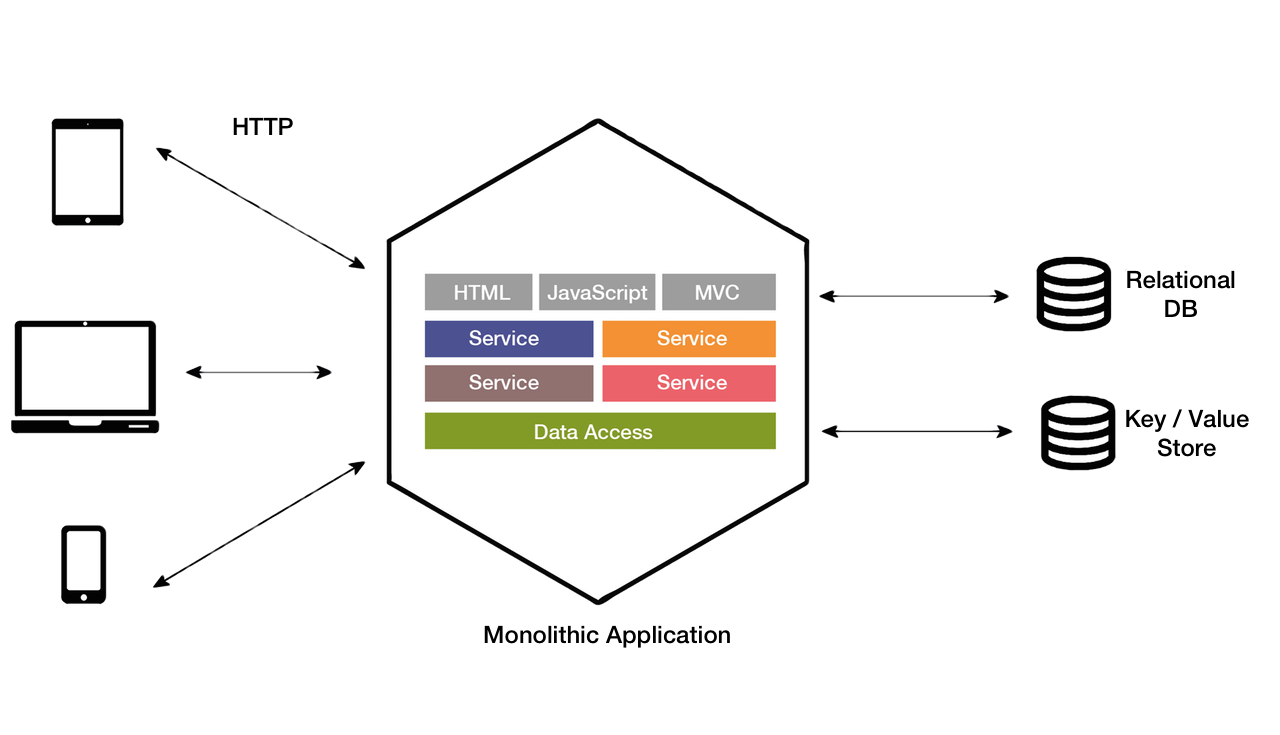
\includegraphics[width=\textwidth/2]{immagini/monolithic_architecture.png} % FONTE: https://medium.com
	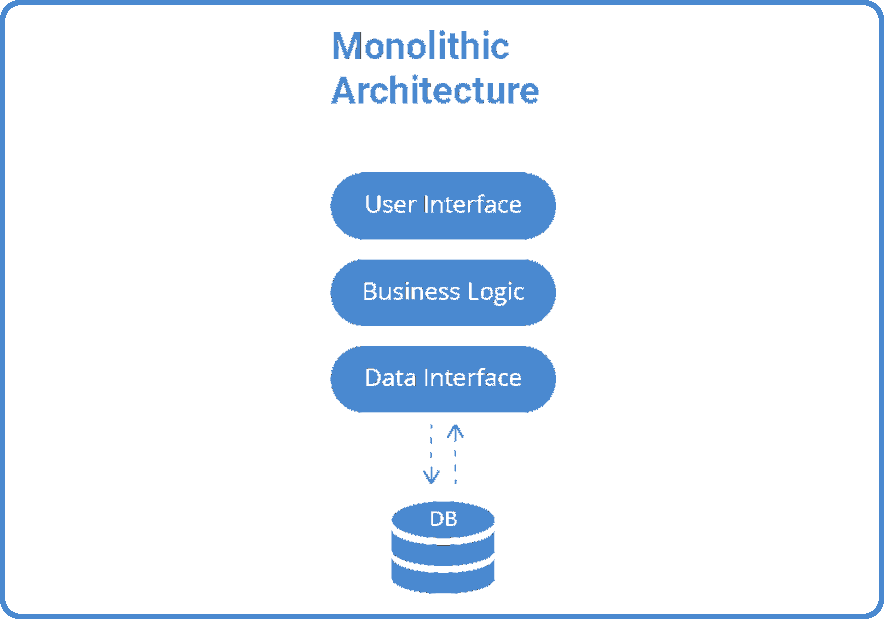
\includegraphics[width=0.28\textwidth]{immagini/monolithic_architectureB.png} % FONTE: https://www.sam-solutions.com/blog/microservices-vs-monolithic-real-business-examples/
	\caption[Architettura monolitica]{Architettura monolitica\footnotemark}
	\label{fig:monolithic-arch}
\end{figure}
\footnotetext{Fonte immagine: \href{https://www.sam-solutions.com/blog/microservices-vs-monolithic-real-business-examples/}{https://www.sam-solutions.com}}

Come è possibile notare dall'immagine, la \textit{business logic}, la gestione dei dati persistenti e la \textit{user interface}, sono racchiusi in un unico grande monolite, termine da cui è stato tratto il nome di questa architettura.

Che tipo di vantaggi può comportare adottare tale architettura?

% https://microservices.io/patterns/monolithic.html

\paragraph*{Sviluppo} Sviluppare un'applicazione monolitica è per natura semplice, poiché tutto ciò che serve è racchiuso in un unico, talvolta grande, progetto, e gli strumenti di sviluppo e/o IDE 
hanno un ottimo supporto in tale contesto.

\paragraph*{Deploy} Fare un \textit{deploy} dell'applicativo, ossia un rilascio, è banale e diretto, poiché è sufficiente ricompilare il progetto (se previsto dallo \textit{stack} tecnologico utilizzato) e rilasciarlo nell'ambiente di produzione.

\paragraph*{Facile da scalare} Per far scalare l'applicazione, è sufficiente farne girare copie multiple, con la possibilità di utilizzare un \textit{load balancer}.

\paragraph*{Testabilità} Facile da testare, poiché si ha il controllo di tutti gli input e gli output, con possibilità di \textit{mocking} dei \textit{layer}
non in fase di \textit{testing}

\bigskip
Veniamo ora agli svantaggi all'approccio monolitico.

\paragraph*{Dimensione intimidatoria} Al crescere delle dimensioni del progetto, diventa sempre più complicato individuare nuovi sviluppatori pronti ad apportare cambiamenti per nuove \textit{release},
viste le considerevoli dimensioni della \textit{code base}.
%Questo per via delle considerevoli dimensioni della \textit{code base}. che in applicazioni a livello \textit{enterprise} sono sempre di spessore non trascurabile.

\paragraph*{Continuous deployment} La pratica del \textit{continuous deployment} non è generalmente praticabile.
Per aggiornare un singolo componente, è necessario rilasciare l'intera applicazione, comportando minuti, se non ore, di totale indisponibilità del
servizio, nel suo complesso.
Per questo va effettuata una rigorosa pianificazione dei rilasci, nei periodi in cui l'applicativo viene usufruito di meno.

\paragraph*{Scalabilità} Mentre risulta facile scalare l'applicazione, non è altrettanto efficacie. Tutti i dati risiedono in un unico, potenzialmente
enorme, \textit{persistence layer}. Quando la mole di dati inizia ad essere
consistente, ogni componente, per ottenere i dati, deve passare attraverso quest'unico layer che comporta un alto traffico di IO, oltre che un attesa dovuta all'attesa del recupero dei dati dall'eventuale \textit{database}.

\paragraph*{Stack tecnologico} L'inizio dello sviluppo di un applicativo monolitico richiede un ``contratto'' a lungo termine con una stack tecnologico limitato. Una volta effettuata la scelta, non sarà possibile cambiare tecnologie per tutto il ciclo di vita del software (a meno che il prodotto non venga riscritto da zero), poiché tutte le componenti sono unite e dipendenti dalle tecnologie iniziali.

Gli svantaggi penalizzano molto fattori che riguardano la scalabilità
e progetti con target su grandi numeri.
Ecco perché negli ultimi anni il paradigma dei microservizi guadagna
sempre più popolarità ed è sulla bocca di tutti.

%\clearpage

% ------------------------------------------------------------------

\subsection{Architettura a microservizi}

Un'architettura a microservizi può essere genericamente vista come
nella figura che segue:

\begin{figure}[H]
	\centering
	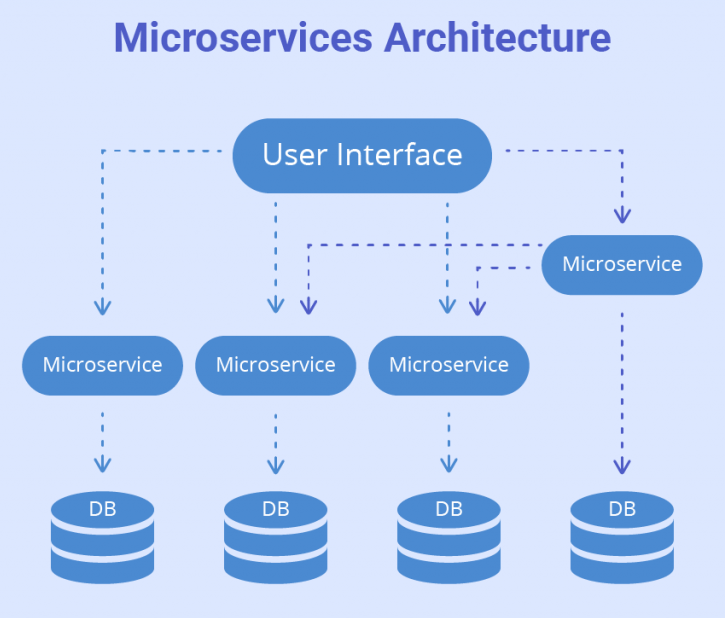
\includegraphics[width=0.8\textwidth]{immagini/microservices_architecture.png} % FONTE: https://www.sam-solutions.com/blog/microservices-vs-monolithic-real-business-examples/
	\caption[Architettura a microservizi]{Architettura  a microservizi\footnotemark}
	\label{fig:microservices-arch}
\end{figure}
\footnotetext{Fonte immagine: \href{https://www.sam-solutions.com/blog/microservices-vs-monolithic-real-business-examples/}{https://www.sam-solutions.com}}

Qui il sistema non è composto da un unico grande monolite, ma viene suddiviso in molti componenti indipendenti, chiamati microservizi poiché contenuti e di limitata responsabilità.
È buona prassi dare a ognuno di essi una singola responsabilità, ove possibile, aderendo al \textit{Single Responsibility Principle}.

Come si può vedere in figura \ref{fig:microservices-arch}, ogni microservizio ha un suo database da cui poter attingere.

Per poter comunicare, ognuno di essi espone delle API, comunemente via HTTP e opzionalmente viene sfruttata una coda di messaggi (e.g. \gloss{Apache Kafka}).

\medskip

Vediamo i vantaggi più salienti di un approccio a microservizi per un applicativo.

\paragraph*{Basso accoppiamento} Uno dei primi vantaggi a cui viene naturale pensare in sistema a microservizi è che mantiene un basso accoppiamento. I servizi, comunicando via HTTP API, sono tra loro totalmente disaccoppiati e indipendenti.

\paragraph*{Manutenzione} La manutenzione, vista la responsabilità e dimensione limitata dei servizi, è di facile approccio.
Non avendo a che fare con \textit{code base} intimorenti come nell'architettura monolitica, scovare e risolvere \textit{bug} richiede
molte meno risorse e tempo, poiché localizzati in un perimetro contenuto.

\paragraph*{Continuous Deployment} La pratica del \textit{continuous deployment} è praticabile con semplicità.
Ogni microservizio può essere rilasciato indipendemente dagli altri,
evitando così la necessità di dover programmare i rilasci che causano l'indisponibilità totale
dell'applicativo per tempo variabile.

\paragraph*{Divisione di business} Dividendo le responsabilità dei microservizi, è possibile dividere totalmente i compiti aziendali in base alle
competenze: chi si occupa di back-end, potrà occuparsi esclusivamente di
back-end, così come chi si occupa di front-end, sviluppo di app per \textit{smartphone}, UI/UX Design etc\dots

\paragraph*{Scalabilità} Uno dei maggiori punti di forza dei microservizi è l'alta scalabilità. La loro natura rende semplice scalare le
applicazioni: nessun servizio avrà una mole di dati enorme da gestire e risponderà in modo rapido. Aggiungendone di nuovi, gli esistenti non vengono rallentati, cosa che invece può accadere aggiungendo funzionalità in un monolite.

\bigskip

Ovviamente, la scelta di tale stile architetturale porta con sé diversi svantaggi che non vanno sottovalutati. Vediamone alcuni.

\paragraph*{Testabilità} Vista la natura distribuita dei microservizi, i test di integrazione e di sistema possono risultare veramente complessi
da attuare. Ad esempio, alcuni servizi potrebbero essere momentaneamente non disponibili, altri con problemi non risolti, invalidando i test.

\paragraph*{Complessità architetturale} I microservizi portano con sé complessità architetturale che in un monolite non c'è.
Con essa, sviluppatori e ingegneri devono tenere conto di molti più fattori, quali:
\begin{itemize}
	\item latenza della rete;
	\item \textit{fault tolerance}: capita spesso che un servizio non sia disponibile. Per questo va previsto un meccanismo di gestione delle
	condizioni di errore;
	\item \textit{message parsing}: per la comunicazione molto spesso vengono usati messaggi in formato JSON.
\end{itemize}

\paragraph*{Comunicazione} Per poter funzionare, i microservizi necessitano di meccanismi per poter comunicare e scambiare messaggi tra loro.

\subsection{Monolite vs. Microservizi: quale scegliere?}
% TODO
Monolite

% ------------------------------------------------------------------

\section{Design pattern per microservizi}

Implementare un'architettura a microservizi non è una pratica semplice:. non è sufficiente dividere il sistema in tanti componenti disaccoppiati per poter dire che un sistema segue questo paradigma.
Vanno seguite le \textit{best practice} delineate da chi si è trovato ad affrontare gli stessi problemi in precedenza.
Tra queste sono stati estrapolati nel corso degli anni diversi \textit{design pattern} per poter raggiungere tale obiettivo.

Segue la discussione solo di alcuni di essi, quelli ritenuti di maggior interesse:

\begin{itemize}
	\item \textit{API Gateway};
	\item \textit{Aggregator};

	\item \textit{Database per service};
	\item \textit{Saga};

	\item \textit{Service discovery};
	\item \textit{Log aggregation};
	\item \textit{Health check};
	\item \textit{Circuit breaker}.
\end{itemize}

% ------------------------------------------------------------------

\subsection{API Gateway pattern}\label{api-gateway}

\paragraph*{Problema} Immaginiamo di avere un applicativo che  che debba supportare diversi tipi di interfaccia utente, quali: 
\begin{itemize}[noitemsep]
	\item una pagina web che utilizza le normali tecnologie del web, quali HTML5, CSS e Javascript;
	\item applicazione Android e iOS.
\end{itemize}

L'applicazione in questione potrebbe mettere a disposizione i seguenti servizi (sotto forma di microservizi):
\begin{itemize}[noitemsep]
	\item servizio informativo;
	\item servizio di login;
	\item servizio di registrazione;
	\item servizio di inventario;
	\item etc\dots
\end{itemize}

%Inoltre il servizio deve esporre via API REST i dati per permettere a software terzi di interagire con tali informazioni.

\begin{figure}[H]
	\centering
	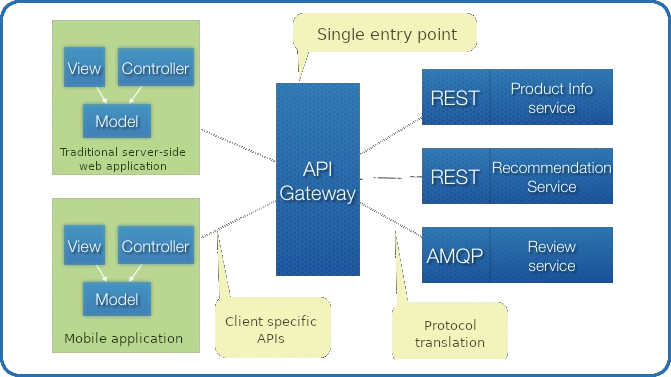
\includegraphics[width=0.8\textwidth]{immagini/apigateway.png}
	\caption[API Gateway]{Esempio d'uso dell'API Gateway pattern\footnotemark}
	\label{fig:api-gateway}
\end{figure}
\footnotetext{Fonte immagine: \url{https://microservices.io/patterns/microservices.html}}

Come possono i vari consumatori dell'app sapere a quale microservizio accedere per una determinata funzionalità?

\paragraph*{Soluzione} Mettere a disposizione un unico punto d'entrata per l'intero sistema, per tutti i \textit{client}.
Questo \textit{entry point} viene chiamato API Gateway.

Esso gestisce le richieste principalmente in due modi:
mappandole verso i servizi che si occupano di quel compito specifico oppure espandendo la singola richiesta a multiple chiamate di vari servizi distinti.

Ci sono almeno un paio di varianti dell'API Gateway:

\begin{itemize}
	\item esporre API diverse, differenziate per tipo di client;
	\item definire un API Gateway differente per ogni tipo di client.
\end{itemize}

% ------------------------------------------------------------------

\subsection{Aggregator pattern}

\paragraph*{Problema} Quando si dividono le funzionalità del \textit{business} in tanti piccoli frammenti logici (i microservizi), è necessario pensare
a come far collaborare i dati ottenuti da ognuno di essi.
Questa non è una responsabilità che può essere lasciata ai consumatori del servizio, anche perché li potrebbe portare a comprendere l'implementazione interna del prodotto, rompendo il principio di \textit{information hiding}.

\paragraph*{Soluzione} L'\textit{Aggregator pattern} si occupa di risolvere questo problema: ``aggrega'' i dati ottenuti dai vari servizi e
manda la risposta finale ai consumatori.

Ci sono due modi di fare ciò:
\begin{itemize}
	\item un microservizio composto che fa le chiamate ai servizi necessari
	unificando e trasformando i dati;
	\item Come detto in precedenza, un \textit{API Gateway} stesso può occuparsi di coprire il ruolo di \textit{aggregator}.
\end{itemize}

% ------------------------------------------------------------------

\subsection{Database per service pattern}

\paragraph*{Problema} Ci sono alcuni concetti da tenere in considerazione quando si va a progettare un sistema a microservizi:
\begin{itemize}[noitemsep]
	\item i servizi vanno tenuti scarsamente accoppiati;
	\item alcune transazioni hanno bisogno di ottenere dati presenti in diversi servizi;
	\item i database hanno bisogno di essere replicati per poter scalare.
\end{itemize}

\paragraph*{Soluzione} Per risolvere i problemi sopra descritti, in fase di progettazione va previsto il paradigma di \textit{database per service}.
I dati persistenti di un servizio non possono essere acceduti direttamente da altri servizi, ma vanno ottenuti tramite le API esposte dal servizio.

% ------------------------------------------------------------------

\subsection{Saga pattern}

\paragraph*{Problema} Immagina di aver applicato il pattern ``database per service''.
A questo punto, i servizi sono scarsamente accoppiati, tuttavia sorge un nuovo problema: alcune funzionalità di \textit{business}, si diffondono su più servizi e serve un meccanismo per garantire la consistenza dei dati
tra i vari servizi. 

Come è possibile mantenere tale consistenza di dati?

\paragraph*{Soluzione} Implementare ogni transazione di \textit{business} come un saga in modo che, qualvolta avvenga una transazione, il saga pubblichi un messaggio o evento che inneschi il prossimo saga nella catena ad effettuare la propria transazione locale, che a sua volta pubblicherà il messaggio di transazione avvenuta.
Dev'essere previsto un meccanismo di ``rollback'' di tutte le transazioni avvenute se una di esse nella catena fallisce, nel caso qualche regola venisse violata.

Ci sono due modi per coordinare il \textit{Saga pattern}:
\begin{itemize}
	\item \textit{Choreography}: ogni transazione locale pubblica un evento che scatena le transazioni locali in altri servizi;
	\item \textit{Orchestration}: un \textit{orchestrator} dice ai partecipanti quali transazioni locali eseguire.
\end{itemize}

\begin{figure}[H]
	\centering
	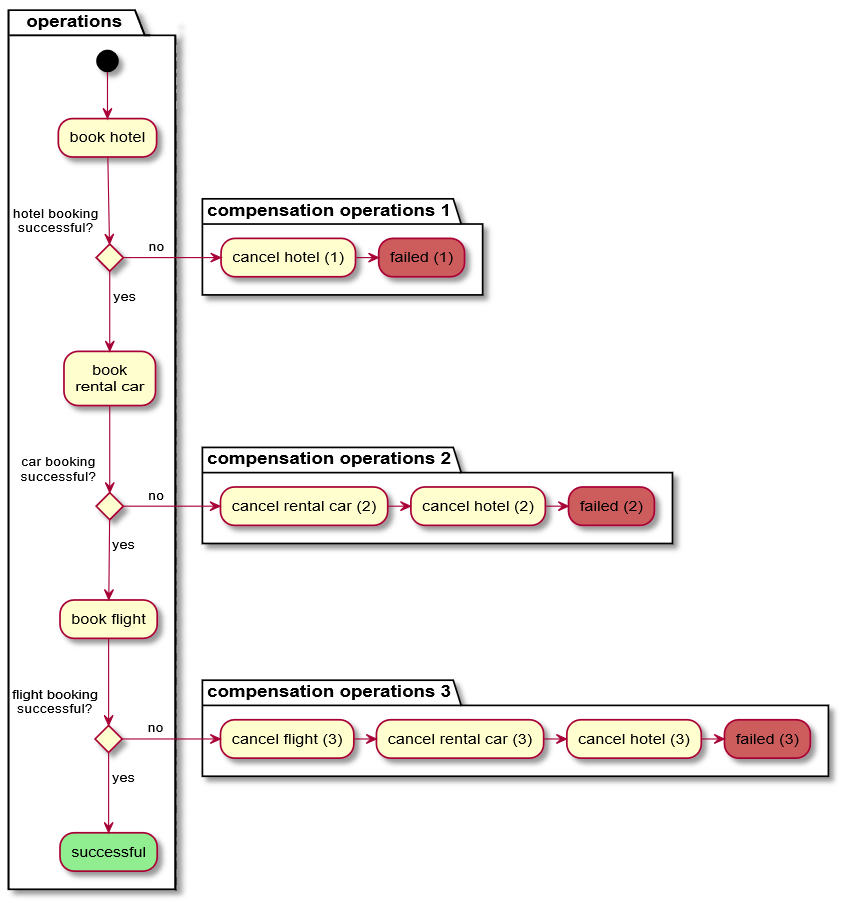
\includegraphics[width=0.8\textwidth]{immagini/saga-example.png}
	\caption[Esempio di Saga pattern]{Esempio di applicazione del Saga pattern\footnotemark}
\end{figure}
\footnotetext{Fonte immagine: \url{https://commons.wikimedia.org}}

% ------------------------------------------------------------------

\subsection{Service Discovery pattern}\label{service-discovery}

\paragraph*{Problema} In un'architettura basata su microservizi, come si può gestire il \textit{routing}, ossia il processo di selezione di un percorso su una rete, che sarà comunemente composta da diverse istanze di più servizi?
Ogni servizio avrà il suo indirizzo (mappato su una porta specifica):  in un sistema distribuito non è ragionevole tenere traccia degli indirizzi manualmente, poiché l'IP di \textit{container} e macchine virtuali è spesso assegnato dinamicamente, cambiando nel tempo.

È necessario avere un processo che si occupi di tenere traccia di tutti i servizi coinvolti nel sistema e permetta di scoprire la loro posizione nella rete.

\paragraph*{Soluzione} Va fornito un \textit{Service Registry} che abbia esattamente questo ruolo:
ogni istanza di ogni servizio che viene inizializzata, va registrata nel \textit{Service Registry}, e ogni istanza non disponibile o eliminata va rimossa dal registro.

\begin{figure}[H]
	\centering
	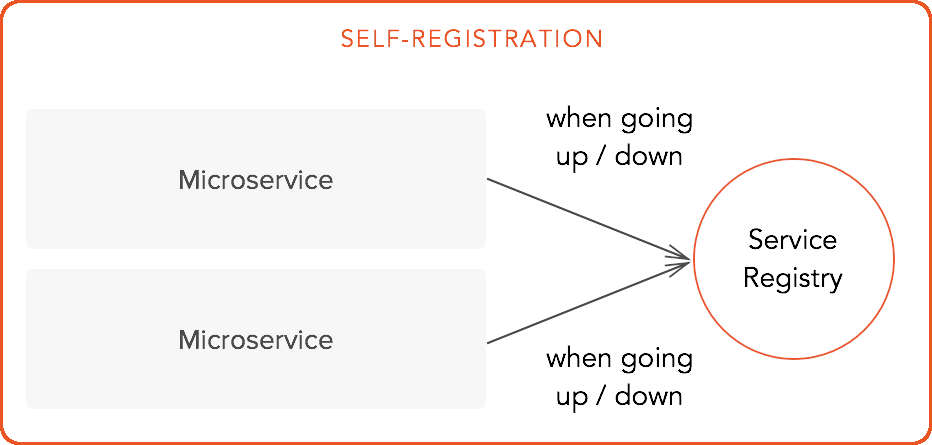
\includegraphics[width=\textwidth]{immagini/service-registry.png}
	\caption[Esempio di Saga pattern]{Service registry\footnotemark}
\end{figure}
\footnotetext{Fonte immagine: \href{https://auth0.com/blog/an-introduction-to-microservices-part-3-the-service-registry/}{https://auth0.com}}

L'attività di ``scoperta'' dei microservizi è chiamata \textit{Service Discovery}. Ne sono presenti due tipi:
\begin{itemize}
	\item \textit{Client-side discovery};
	\item \textit{Server-side discovery}.
\end{itemize}
Alcuni esempi saranno discussi in \S\ref{cap:spring-cloud}.

% ------------------------------------------------------------------

\subsection{Circuit Breaker pattern}\label{circuit-breaker}

\paragraph*{Problema}

\paragraph*{Soluzione}